\documentclass[a4paper,UKenglish,cleveref, autoref, thm-restate]{lipics-v2021}
\usepackage{xspace}
\usepackage{graphicx} % For \includegraphics
%\graphicspath{{./graphics/}}%helpful if your graphic files are in another directory
\usepackage{amsmath}
\bibliographystyle{plainurl}% the bibstyle
\usepackage{cleveref} % Provides \Cref


\title{Instructions for Formal Verification 2020 Reports} %TODO Please add

\titlerunning{} %TODO optional, please use if title is longer than one line

\author{Romain Edelmann}{EPFL}{romain.edelmann@epfl.ch}{}{}
\author{Viktor Kun\v{c}ak}{EPFL}{viktor.kuncak@epfl.ch}{https://orcid.org/0000-0001-7044-9522}{}

\authorrunning{R.~Edelmann and V.~Kun\v{c}ak}

\Copyright{Romain Edelmann and Viktor Kun\v{c}ak} %TODO mandatory, please use full first names. LIPIcs license is "CC-BY";  http://creativecommons.org/licenses/by/3.0/

\ccsdesc[500]{Software and its engineering~Software verification and validation}

\keywords{formal verification, theorem proving, concurrency, decision procedure} %please add comma-separated list of keywords relevant to your project

\category{}
\relatedversion{}
\supplement{}
\nolinenumbers 
\hideLIPIcs

\begin{document}

\maketitle

\begin{abstract}
  This meta-circular report explains how to write a report
  for the Formal Verification course.  To write this
  abstract, we have first written an initial version of
  it. Then, after the rest of the report was complete, we
  revised the abstract to make sure that it contains the
  most important points. As part of this revision, we have
  concluded that we did not set as great of an example as we
  hoped, but may have shown some simple latex commands and
  expected section structures.
\end{abstract}

\definecolor{bgcolor}{RGB}{240,252,210}
\definecolor{kwcolor}{RGB}{0,0,200}
\lstdefinelanguage{scala}{
  keywordstyle=\color{kwcolor},
  backgroundcolor=\color{bgcolor},
  alsoletter={@,=,>},
  morekeywords={abstract, case, class, def,
        else, extends, false, free, if, implicit, match,
        object, true, val, var, while, sealed,
        for, dependent, null, type, with, try, catch, finally,
        import, final, return, new, override, this, trait,
        private, public, protected, package, throw},
  sensitive=true,
  morecomment=[l]{//},
  morecomment=[s]{/*}{*/},
  morestring=[b]",
  mathescape=true,
  %emph={Int,Char,Boolean,String,Unit},
  %emphstyle={\color{blue}}
}
\lstset{language=scala}


\section{Introduction}
\label{sec:intro}

This topic of this report sits at the intersection of two
areas: formal verification as the subject line, and the
general topic of writing a scientific report in computer
science. That said, please keep in mind that this is not a
serious report whose contents is meant to be taken overly
seriously, but rather a report template that shows how to
use latex to typeset your report.

\subsection{Formal verification.}
Formal verification is computer science subject in at least
two aspects: it applies rigorous analysis to
\emph{computer systems} % you can make short or long lines, latex decides how to arrange words into paragraphs for you
% \emph stands for emphasis
(thus, computing is its subject), and it uses
algorithms and their implementations in tools to help
automate this task (thus, computing is a tool to make the
task more feasible). In principle, it is possible to do
formal verification manually, and early formal methods such
as the Z notation focused on specification and manual proofs
\cite{DBLP:books/daglib/0072139}.
% did you see that \cite above? It refers to an identifier in main.bib file.
Today we expect some
degree of \textbf{automation} from specification and verification
process. % normally we do not use bold fonts very often, but this was important

Among main directions for automation in formal verification are:
\begin{enumerate}
\item building better theorem provers, advancing SMT solvers, SAT solvers, and first-order theorem provers
\item building methods to infer inductive invariants, such as abstract interpretation
\item designing type inference mechanisms and tactics for proof assistants
\end{enumerate}
Thanks in part to student projects, we were able to see aspects of all of these directions.

\subsection{Report formats}
Journal and conference proceedings publishers tend to
specify formatting instructions for their contributions,
such as Dagstuhl Publishing proceedings instructions\footnote{\url{https://submission.dagstuhl.de/documentation/authors}.
  It is better to not use URLs if you can provide a citation entry instead. Also, avoid lengthy footnotes in general.
  If the footnote is long, it distracts the reader in two ways: first, visually, because they have to skip to the bottom
  of the page and then go back. It is also bad in terms of readers' focus, because it often involves a digression.
  Digressions are best avoided, because the reader tends to forget what the main point of the text was. On top of all that,
  LaTeX tends to split very long foonotes across multiple pages, which makes reading them almost as bad as footnotes in books.
  If not, then a large footnote occupies a large portion of the bottom of a page, which does not look good. Footnotes also
  have too small font, so they are hard to read.
  In summary, it is best to avoid footnotes, and avoid long ones entirely by restructuring the text to make the remarks
  appear inline or not at all.}
% The above was a long foonote, in case you did not notice!
% This current line, of course, is a comment that will not appear in the document.
% LaTeX has no nested comments.
on which this very report is based, but typically the publishers
leave the content of the articles to the reviewers,
editors, and mentors who provide initial advice for
scientific writing.

\subsection{Prior work}

We would cite here the main work on which we build our solution. We should clarify why
previous solutions do not solve the problem we were aiming to solve, or at least why
we think we could not google the solution.

\subsection*{Our approach} % the star makes the section number disappear

\begin{remark}
Scientific communication is part
of a larger area of communication studied in humanities
departments throughout the world, but we have not pursued these studies, so we cannot comment on the overlap of concepts learned
there with the specific subject of scientific reporting, which scientists, somewhat arrogantly, tend to believe has mostly
to do with science and not with reporting.
\end{remark}

We are now ready to state the main rationale behind this report. % ends with a period . not a colon :
\begin{proposition}\label{prop:main} % the identifier prop:main can have ':' inside but that's just a naming convention
  Content is ultimately more important than the presentation, but adopting certain presentation conventions
  gives the author an easily gained advantage that may positively bias the readers and may help them accept author's ideas.
  % It's hard to spell favourable. But latex file is a text file and spell checking mostly works.
  % emacs has spell checking modes that will not complain about latex commands like \emph and thus be less annoying to use
  % Apparently there exists also languagetool that can help with grammar, if you can get it to work.
\end{proposition}

The main challenges in writing the report sample is that it should not be too long or too confusing.
Another challenge is that it may be written in a relatively short period of time, though this aspect
may well be shared by actual reports.

\subsection*{Contributions} % the star makes the section number disappear
In summary, in this report we have taken a hopefully decent-looking non-copyrighted template for proceedings
and wrote an example file.

The main contributions of this report are the following:
\begin{enumerate}
\item We illustrate how to use latex, though we hope that this is a skill already acquired. If not, once can consider
  vast LaTeX literature~\cite{latexTutorial}.
\item We suggest a list of sections.
\item We make various remarks that serve primarily to fill the space.
\end{enumerate}

\section{Example}
\label{sec:example}

In this example section, we show how to our system works. It
is a good to start a section with a short sentence (such as
previous one) stating the purpose of that section, before
continuing with any other remarks.

An example section is very helpful. It should give the
reader the feeling for \emph{what} your work accomplishes,
without going into details of \emph{how} it does it.

We have built a verification system (once upon a time, in 2006). Figure~\ref{fig:session} shows an example of a verification session.
\begin{figure}
  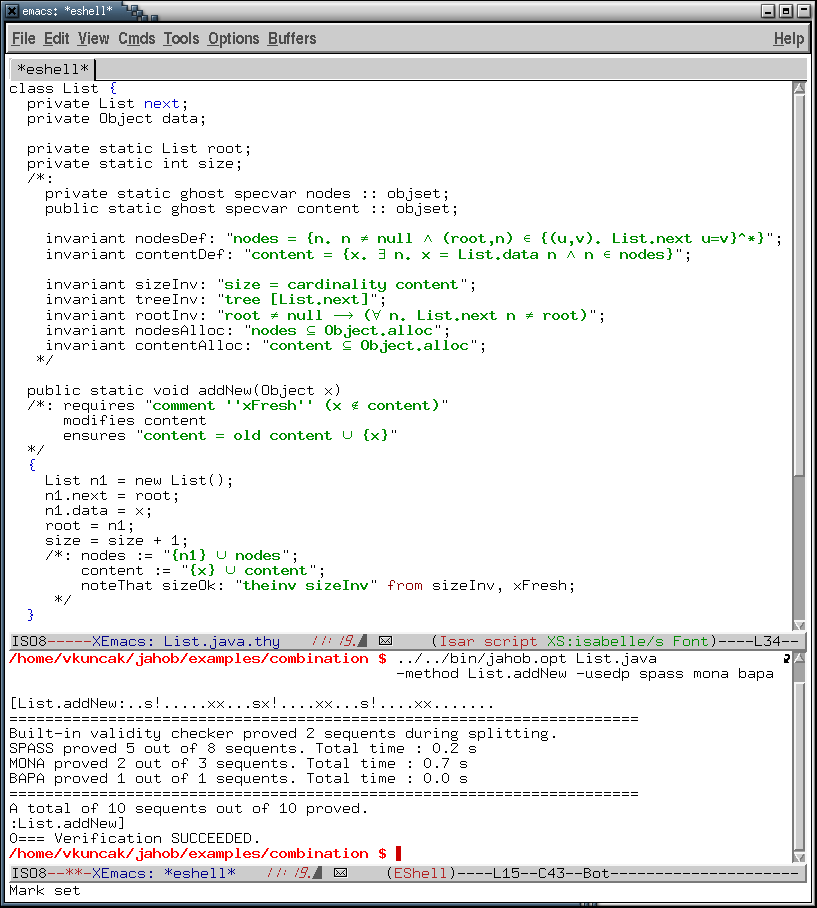
\includegraphics[width=\textwidth]{screenshot.png}
  \caption{A screenshot of a verification session.\label{fig:session}}
\end{figure}

\section{Overview}

By year 2006, one of the authors, together with
collaborators, build a verification system called
Jahob. Figure~\ref{fig:overview} shows an overview of this
system. Different aspects of the system are outlined in the
thesis~\cite{Kuncak07DecisionProceduresModularDataStructureVerification}.

\begin{figure}
  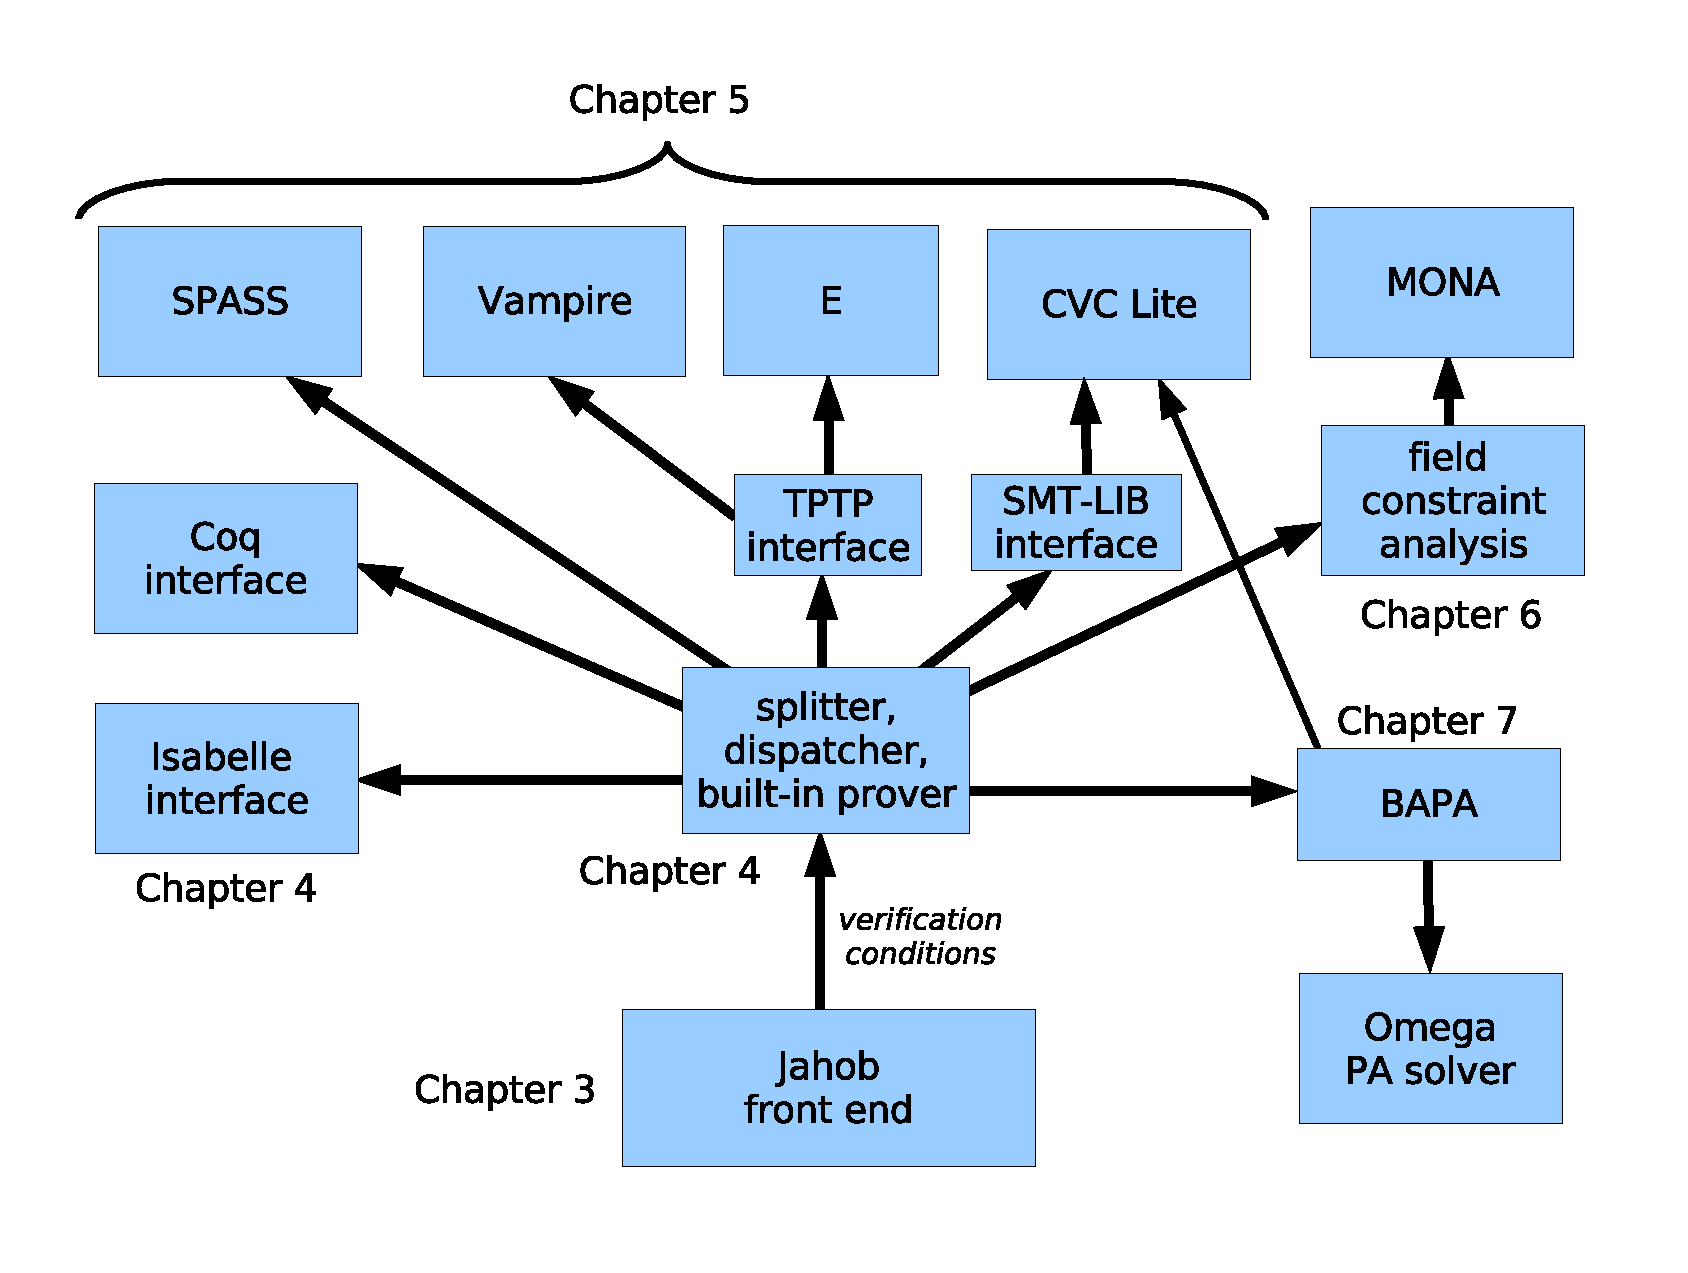
\includegraphics[width=0.9\textwidth]{system-diagram.eps} % you can also write e.g. [scale=0.3] instead of width=
  \caption{An Overview of the Jahob Verification System\label{fig:overview}}
\end{figure}

\section{A Solver}

In this section, we explain the solver we built.
This would be a sketch of a more technical section.

For the sake of illustration, Figure~\ref{fig:dpll} shows a
pseudo code of a SAT solver based on DPLL
procedure~\cite{10.1145/321033.321034}.
\begin{figure}
  \newcommand{\BB}{Bool} % this macro is used in the listing in file DPLL.scala, included below
  % It is safer to put a listing into a separate file and include it like this:
  \lstinputlisting[language=scala]{DPLL.scala} % you will see DPLL.scala is not quite Scala due to some $...$ escapes
  \caption{This figure should show something new and interesting but, for illustration pruposes, it is merely a sketch
    of a DPPL algorithm for SAT that should be familiar from Lecture 3.\label{fig:dpll}}  
\end{figure}

Note that the above algorithm is simplified in several respects:
\begin{itemize}
\item It uses mathematical sets to store clauses. This is very inefficient
\item It uses non-deterministic constructs such as selecting an element from the set. It thus leaves the policy on how to do actual selection under-specified.
\end{itemize}
In the rest of this report we could see how to make it more efficient (though we will, in fact, not).
We present a part of the search procedure used in actual CafeSAT code in Appendix~\ref{app:verifiedFunction}.

\section{Implementation}

We have implemented our approach in ocaml. Our system is available in the following repository:
\begin{center}
  \url{https://github.com/epfl-lara/jahob}
\end{center}
and build instructions are in file \verb|README.md| in the top-level directory.

\section{Experimental Evaluation}

We have evaluated our solver on benchmarks taken from standard benchmark suites~\cite{DBLP:conf/fm/HojjatKGIKR12,
  Sut17,
  BarFT-SMTLIB,
  10.1007/978-3-030-45237-7_21}
  
We have selected only those benchmarks that portray our
solver in good light. To make our results look more
convincing, we have added some benchmarks that our solver
cannot solve (and also no other solver can solve, because
they encode open conjectures in number theory).\footnote{You should adopt a more convincing
  approach to evaluation if possible. For a short project, make it clear that you understand
  where your limitations are, rather than pretending they do not exist. Also, do not use footnotes.}

\section{Related Work}

In this section we argue that we are very well aware of the previous work in the area.
This may be more or less realistic for a project report in a course, but is crucial for reports that
reflect a longer piece of work.

Dependent types are very popular approach in programming language community \cite{fakingIt}; a title
that is a good reflection of the superficial nature of this very report sample.
Often the idea is that some forms of type dependency are easy, and general form of type dependency
allows us to prove complex properties. From this the reader should get the hint that using dependent
types makes verification easy. In reality, verification is never easy; it is merely the only way
to have high confidence that software is correct.

Types that refine type systems of languages such as Haskell and ocaml with predicates demonstrate
an appealing combination between automation and expressive power \cite{10.1145/2858949.2784745}. They appear
to have been used to prove properties somewhat simpler than those used in Stainless case studies
\cite{HamzaETAL19SystemFR}, but have advantage in inferring properties that are not inductive
yet fit the provided invariant templates.

\section{Future work}

In this section we point out to those aspects that we would have liked to explore had there been
more time. We will be careful not to say too much that can be used against us and, where aspects
are left unfinished, there were specific technical challenges that we encountered, beyond the lack
of time (which is always a problem).

In terms of this report itself, there is only so much that
one can do in a short amount of time in illustrating what a
report should look like. Thus, we encourage students to contact
us for feedback on initial versions of the report, so that we can
point out to specific ways in which it can be improved.

\section{Conclusions}

Admittedly, it would have been possible to write a detailed
treatise on how to write reports. However, we hope that the
following example will already streamline the format and set
some expectations on how the report should look like in its
form and structure, despite the lack of substance and
admittedly confusing nature of the matter.

\vspace{0.5cm} % somem vertical space since we are creating this paragraph manually
\noindent % otherwise many styles like to indent the first word of a paragraph
\textbf{\large Acknowledgements.}\ % Bold, large font
The authors of this report would like to thank the funding agencies such as Swiss Science Foundation, as well as EPFL,
  for creating a wonderful environment where teaching and research can co-exist in synergy.
  The authors thank their parents, primary school teachers, as well as their undergraduate and doctoral advisors
  for improving their writing skill, as well as science camp instructors and professors at the undergraduate
  study for fostering their interest in logic and functional programming. The authors also
  thank students in the course and hope that they will consider future projects with our lab.

% =======================================================================================

\bibliography{main} % this will make bibliography appear

% =======================================================================================
\appendix % from now on, sections will appear as appendices

\section{Appendix: Listing of our main verified function}\label{app:verifiedFunction}

This appendix lists the full function whose fragments we only briefly sketched in Section~\ref{sec:example}.

\lstinputlisting[language=scala]{DPLL-Full.scala} % you will see DPLL.scala is not quite Scala due to some $...$ escapes

It may appear that we have verified a SAT solver. In fact, we have not done so ourselves.
Others, however, have successfully generated code from SAT solver formalizations inside Isabelle/HOL proof assistant
\cite{DBLP:conf/cade/BlanchetteFW16}. Now we just cited a paper in an appendix. If it was important for this report,
it would have been better to cite it inside the main body of the paper.

We should not use appendix just to make it look like we have a detailed report. In fact, we should instead link to a git repository.
For example, the code snippet above is available from here:
\begin{center}
  \url{https://github.com/regb/cafesat/blob/77f3c582f7b8baaf20596c08cb689508ccf0a306/src/main/scala/cafesat/sat/Solver.scala}
\end{center}
As you may know from reading github documentation, you can refer to the current version of the file, or, like above, to
a specific commit that will not change unless you rewrite history after accidentally committing a password into git.

\section{Appendix: Additional Information}\label{app:correctness}

Here we could present, for example, additional experiments
that did not fit into the length of the main paper.  If we
do not have a page limit, the only reason to have appendices
is when your report is too long for your readers and you
wish to provide additional information that may be helpful
for someone going into depth, but that is better presented
as a report than as some files in a git repository (or is
too important to be left only in a git repository).


\end{document}
